\newcommand{\orgmode}{\texttt{org mode}}
\newcommand{\Makefile}{\mintinline{shell}{Makefile}}
\newcommand{\context}{\mintinline{shell}{context}}
\newcommand{\CC}{C\nolinebreak\hspace{-.05em}\raisebox{.4ex}{\tiny\bf +}\nolinebreak\hspace{-.10em}\raisebox{.4ex}{\tiny\bf +}}
\def\CC{{C\nolinebreak[4]\hspace{-.05em}\raisebox{.4ex}{\tiny\bf ++}}}

\section{Introduction}


The ultimate goal of \ac{QMCkl} is to provide a high-performance
implementation of the main kernels of \ac{QMC}. In this particular
\ac{WP}, we focus on the definition of the \ac{API}, the tests,
and on a \emph{pedagogical} presentation of the algorithms.  We expect
the \ac{HPC} experts to use this repository as a reference for re-writing
optimized versions of the functions described in this library, using
the same \ac{API}.

The documentation of the current status of the library is available
at \url{https://trex-coe.github.io/qmckl}, and the source code is
available on the GitHub repository at \url{https://github.com/trex-coe/qmckl}.


\subsection{Literate programming}

In a traditional source code, most of the lines of source files of a
program are code, scripts, {\Makefile}s, and only a few lines are
comments explaining parts of the code that are non-trivial to
understand. The documentation of the prorgam is usually written
in a separate directory, and is often outdated compared to the code.

Literate programming\cite{knuth_1992} is a different approach to
programming, where the program is considered as a publishable-quality
document. Most of the lines of the source files are text,
mathematical formulas, tables, figures, \textit{etc}, and the lines of
code are just the translation in a computer language of the ideas
and algorithms expressed in the text. More importantly, the ``document'' is
structured like a text document with sections, subsections, a bibliography,
a table of contents \textit{etc}, and the place where pieces of code
appear are the places where they should belong for the reader to
understand the logic of the program, not the places where the compiler
expects to find them. Both the publishable-quality document and the
binary executable are produced from the same source files. 

Literate programming is particularly well adapted in this context, as
the central part of this project is the documentation of an
\ac{API}. The implementation of the algorithms is just an expression
of the algorithms in a language that can be compiled, so that the
correctness of the algorithms can be tested.

We have chosen to write the source files in {\orgmode}
format,\cite{schulte_2012} as any text editor can be used to edit
{\orgmode} files. To produce the documentation, there exists multiple
possibilities to convert {\orgmode} files into different formats such
as \ac{HTML} or \ac{PDF}. The source code is easily extracted from the
{\orgmode} files invoking the Emacs text editor from the command-line in the
{\Makefile}, and then the produced files are compiled.
Moreover, within the Emacs text editor the source code blocks can be
executed interactively, in the same spirit as Jupyter notebooks.\cite{Kluyver_2016}

\section{Source code}

\subsection{Choice of the programming language}

Most of the codes of the \ac{TREX} \ac{CoE} are written in Fortran
with some scripts in Bash and Python. Outside of the
\ac{CoE}, Fortran is also important (Casino, Amolqc), and other
important languages used by the community are C and {\CC} (QMCPack,
QWalk), and Julia is gaining in popularity.\cite{poole_2020} The
library we design should be compatible with all of these languages.
The \ac{QMCkl} \ac{API} has to be compatible with the C language
since libraries with a C-compatible \ac{API} can be used in every
other language.

High-performance versions of the \ac{QMCkl}, with the same \ac{API},
will be rewritten in \ac{WP}~3 by the experts in \ac{HPC}. These
optimized libraries will be tuned for specific architectures, among
which we can cite x86 based processors, and \ac{GPU} accelerators.
Nowadays, the most efficient software tools to take advantage of
low-level features of the processor (intrinsics) and of \acp{GPU} are
for {\CC} developers. It is highly probable that the optimized
implementations will be written in {\CC}, and this is agreement with our
choice to make the \ac{API} C-compatible.

Fortran is one of the most common languages used by the community, and
is simple enough to make the algorithms readable both by experts in
\ac{QMC}, and experts in \ac{HPC}. Hence we propose in this
pedagogical implementation of \ac{QMCkl} to use Fortran to express the
QMC algorithms. As the main languages of the library is C, this
implies that the exposed C functions call the Fortran routine.
However, for internal functions related to system programming, the C
language is more natural than Fortran.

The  Fortran  source  files  should provide  a  C  interface  using the
\mintinline{Fortran}{iso_c_binding} module. The name of the Fortran source files
should end with \mintinline{shell}{_f.f90} to be properly handled by the
{\Makefile}.  The names of the functions defined in Fortran should be the
same as those exposed in the \ac{API} suffixed by \mintinline{shell}{_f}.
Fortran interfaces should also be written in the
\mintinline{shell}{qmckl_f.f90} file.

\section{Design of the library}

The proposed \ac{API} should allow the library to deal with memory
transfers between CPU and accelerators, and to use dynamically
different levels of floating-point precision.  We chose a
multi-layered design with low-level and high-level functions (see
below).

\subsection{Naming conventions}

To avoid namespace collisions, we use \mintinline{C}{qmckl_} as a prefix for
all exported functions and variables.  All exported header files
should have a file name prefixed with \mintinline{shell}{qmckl_}.

For instance, if the name of the {\orgmode} file is
\mintinline{shell}{xxx.org}, the name of the produced C files should
be \mintinline{shell}{xxx.c} and \mintinline{shell}{xxx.h} and the
name of the produced Fortran file should be
\mintinline{shell}{xxx.f90}

Arrays are in uppercase and scalars are in lowercase.

In the  names of  the variables and  functions, only the singular
form is allowed.

\subsection{Application programming interface}

In the C language, the number of bits used by the integer types can
change from one architecture to another one. To circumvent this
problem, we choose to use the integer types defined in
\mintinline{C}{<stdint.h>} where the number of bits used for the
integers are fixed.

To ensure that the library will be easily usable in \emph{any} other
language than C, we restrict the data types in the interfaces to the
following:
\begin{itemize}
\item 32-bit and 64-bit integers, scalars and and arrays
  (\mintinline{C}{int32_t} and \mintinline{C}{int64_t})
\item 32-bit and 64-bit floats, scalars and and arrays
  (\mintinline{C}{float} and \mintinline{C}{double})
\item Pointers are always casted into 64-bit integers, even on legacy 32-bit architectures
\item ASCII strings are represented as a pointers to character arrays
  and terminated by a zero character (C convention).
\item Complex numbers can be represented by an array of 2 floats.
\item Boolean variables are stored as integers, \mintinline{C}{1} for
\mintinline{C}{true} and \mintinline{C}{0} for \mintinline{C}{false}
\item Floating point variables should be by default
\mintinline{C}{double}, unless explicitly mentioned
\item integers used for counting should always be \mintinline{C}{int64_t}
\end{itemize}

To facilitate the  use in other languages than C, we will provide some
bindings in other languages in other repositories.


\subsubsection{Global state}

Global variables should  be avoided in the library,  because it is
possible that one  single program needs to  use multiple instances
of the library. To solve this  problem we propose to use a pointer
to a {\context}  variable,  built   by  the  library   with  the
\mintinline{C}{qmckl_context_create} function. The
{\context} contains the global state of the library, and is used as
the first argument of many \ac{QMCkl} functions.

The internal structure of the {\context}  is not specified, to give a
maximum of  freedom to  the different  implementations.  Modifying
the  state   is  done   by  setter   and  getter functions,   prefixed  by
\mintinline{C}{qmckl_context_set_}  an
\mintinline{C}{qmckl_context_get_}.
When a {\context} variable is modified by a setter, a copy of the old
data structure is made and updated, and the pointer to the new data
structure is returned, such that the old contexts can still be
accessed.  It is also possible to modify the state in an mutable
fashion, using the \mintinline{C}{qmckl_context_update_} functions.
The {\context} and its old versions can be destroyed with
\mintinline{C}{qmckl_context_destroy}.


\subsubsection{Low-level functions}

Low-level functions are very simple  functions which are leaves of
the function call tree (they don't call any other \ac{QMCkl} function).

These  functions   are   \emph{pure},   and  unaware   of   the   \ac{QMCkl}
{\context}. They are not allowed to allocate/deallocate memory, and
if they need temporary memory it should be provided in input.

\subsubsection{Numerical precision}

The number of bits of precision  required for a function should be
given as an input of low-level computational functions. This input
will be used to define the values of the different thresholds that
might be  used to  avoid computing unnecessary  noise.  High-level
functions  will  use  the  precision specified  in  the  \texttt{context}
variable.

\subsubsection{High-level functions}

High-level functions  are at  the top of  the function  call tree.
They  are  able  to  choose which  lower-level  function  to  call
depending on the required precision, and do the corresponding type
conversions.  These functions are  also responsible for allocating
temporary storage, to simplify the use of accelerators.

The high-level  functions should be pure,  unless the introduction
of non-purity is justified. All the side effects should be made in
the \texttt{context} variable.


\subsection{Algorithms}

Reducing the scaling of an  algorithm usually implies also reducing
its arithmetic  complexity (number  of flops per  byte). Therefore,
for  small  sizes   \(\mathcal{O}(N^3)\)  and  \(\mathcal{O}(N^2)\)
algorithms are  better adapted than linear  scaling algorithms.  As
\ac{QMCkl} is a  general purpose library, multiple  algorithms will be
implemented adapted to different problem sizes.



\section{Documentation of the API}

In this section, we include the documentation of the library which is
automatically generated from the {\orgmode} files, in the current status.
The library is still at an early development stage. Up to now most of
the effort was made on preparing solid bases for the development of
the library, more related to system programming than scientific
programming (the context variable, memory allocation, conventions,
Makefiles, generation of the documentation, \textit{etc}). The actual
implementation of the kernels is in progress, and we refer the
reaer to section~\ref{sec:codesign} for more detail on our strategy.

% TODO : include here documentation

\section{Co-design}
\label{sec:codesign}

Research codes are developed over a long period of time by multiple
researchers, Ph.D students and post-docs. The professional evaluation
of these people is based on their scientific production and not on the
quality of the software they write, so code quality and refactoring is
often left in the low-priority tasks. As a consequence, old research
codes often depend on some choices made at an immature stage of the
program, and solutions to bypass these wrong choices make the code
complicated to understand for external people, especially if they are
not familiar with the domain.

\subsection{Kernel extraction}

The strategy we have chosen to extract the kernels of the codes is to
first discuss among the developers of \ac{QMC} codes how they have
implemented a particular kernel. Once the developers have agreed on
which algorithm is best, they first formulate the algorithm in terms
of mathematical expressions in a {\LaTeX} file, and they create a prototype application 
(the \emph{mini-application}) implementing \emph{only} the kernel of
interest. This mini-application can be easily compiled and executed,
and is considered valid when it reproduces exactly the values obtained
with the kernel present in the original \ac{QMC} code.

The mini-app is then thoroughy modified in discussion with the
\ac{HPC} experts of \ac{WP}3 until the optimal data strtuctures are
determined. This step is crucial to facilitate the access to performance
in the \ac{HPC} versions of the library that will be developed in \ac{WP}3.
Once the \ac{QMC} and \ac{HPC} specialists have agreed
on the data structures, the kernel is ready to be implemented in the
library.


\subsection{A concrete example}

The first kernel we have been working on is the three-body component of
the Jastrow factor, which is one of the potential bottlenecks of
extreme-scale calculations that will run on exascale machines.
In the CHAMP program, it is expressed as

\newcommand{\Jeen}{J_{\text{een}}}
\newcommand{\Nel}{N_{\text{elec}}}
\newcommand{\Nat}{N_{\text{nucl}}}
\newcommand{\Nord}{N_{\text{nord}}}
\newcommand{\lmax}{p-k-2\delta_{k,0}}
\newcommand{\br}{\mathbf{r}}
\newcommand{\bR}{\mathbf{R}}
\[
  \Jeen (\br,\bR) = \sum_{\alpha=1}^{\Nat} \sum_{i=1}^{\Nel} \sum_{j=1}^{i-1}
\sum_{p=2}^{\Nord} \sum_{k=0}^{p-1}
\sum_{l=0}^{\lmax} c_{lkp\alpha}
\left( {r}_{ij} \right)^k
\left[ \left( {R}_{i\alpha} \right)^l + \left( {R}_{j\alpha} \right)^l \right]
\left( {R}_{i\,\alpha} \, {R}_{j\alpha} \right)^{(p-k-l)/2} 
\]
where
$\Nel$ is the number of electrons, 
$\Nat$ is the number of nuclei,
$\Nord$ is the maximum order of the polynomial, 
$\br$ contains rescaled electron-electron distances, 
$\bR$ contains rescaled electron-nucleus distances,
and $c_{lkp\alpha}$ are the variational parameters which are non-zero
only when $p-k-l$ is even.

For \ac{QMC} simulations, the first and second derivatives of $\Jeen$ with
respect to the electron coordinates are also required. To optimize the
parameters, the derivative with respect to $c_{lkp\alpha}$
should also be available, and in the context of molecular dynamics or
geometry optimization the first derivatives with respect to $\bR$ are
also required. To compute these derivatives, multiple intermediates
will be common and we need to identify them such that the same
intermediates can be reused for several derivatives.

The mini-application, available on
GitHub\footnote{https://github.com/trex-coe/irpjast} has allowed us to
rewrite the expression in a way allowing us to take advantage of BLAS3
matrix multiplication. The expression is now expressed in terms of
rank-3 and rank-4 tensors \newcommand{\tr}{\mathtt{r}}
\newcommand{\tR}{\mathtt{R}}
\newcommand{\tP}{\mathtt{P}}
\[
  \Jeen(\br,\bR) = 
  \sum_{p=2}^{\Nord}\sum_{k=0}^{p-1}
  \sum_{l=0}^{\lmax} 
    \sum_{\alpha=1}^{\Nat}
    \sum_{i=1}^{\Nel}
    c_{lkp\alpha}\, {\tR}_{i,\alpha\,l}\,
  {\tP}_{i,\alpha,k,(p-k+l)/2}
  \]
with 
  \[
  {\tP}_{i, \alpha, k, l} = \sum_{j=1}^{\Nel} {\tr}_{i,j,k}\,{\tR}_{j,\alpha,l}
  \]
  
This rewriting allowed us to move the computationally intensive part in
$\mathcal{O}(\Nat{\Nel}^2)$ into a BLAS3 matrix multiplication, the
remaining part being in $\mathcal{O}(\Nat \Nel)$.
\begin{figure}[t]
  \begin{center}
  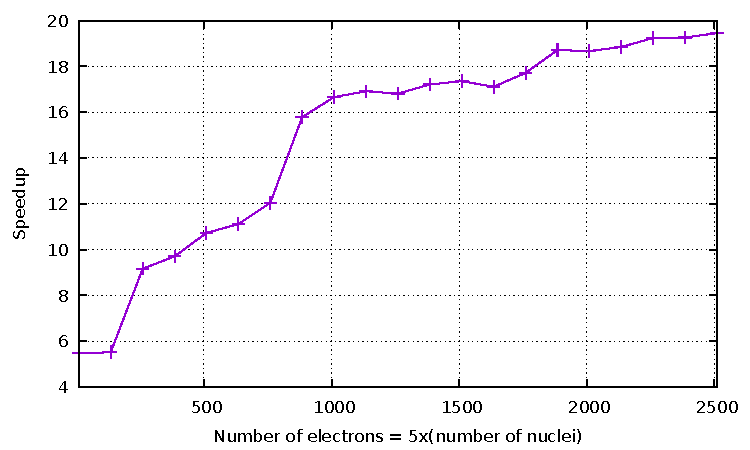
\includegraphics[width=0.75\textwidth]{speedup.pdf}
  \end{center}
  \caption{\label{fig:speedup}Speedup obained after the re-expression of the three-body
    Jastrow factor.}
\end{figure}
The speedup is presented in figure~\ref{fig:speedup}. Further
optimizations will be made on the $\mathcal{O}(\Nat \Nel)$ part before
the kernel will be implemented in \ac{QMCkl}.
The same strategy for kernel extraction of the codes will be applied
to all other possible computational bottlenecks.


\section{License}

The library is licensed under the open-source 3-clause BSD license to facilitate
its adoption in all quantum chemistry software, commercial or not.

\section{Dependencies}

Dependencies are critical: if a user is not able to install the
required dependencies, the user is not going to be able to use our
library, and solving the problem is out of our control. So the list of
external dependencies should be kept as small as possible. 
External libraries should be used \emph{only} if their use is
strongly justified, and if we are sure that the users will be able to
have access to them.

The dependencies needed to use pre-compiled versions of the library
are \ac{BLAS} and \ac{LAPACK}.

The dependencies needed to compile the code are
a C and a Fortran compiler, GNU make, \ac{BLAS} and \ac{LAPACK}, and
$\mu$nit\cite{munit} for building the unit tests.

The dependencies needed to create the \ac{HTML} documentation are
Emacs~26 and the package Emacs-htmlize.


\section{Continuous integration}

Continuous integration has been setup on the GitHub platform. Upon
pull request, the repository is automatically cloned on a virtual
machine. The source code is then extracted from the {\orgmode}
files and the library is compiled. Then the unit tests are compiled
and linked together with the library. If all the tests pass, the
pull request is considered valid, and can be merged.

When the code is updated, the documentation is automatically built and
the server hosting the documentation is updated, such that the web
site containing the documentation is always synchronized with the
latest version of the master branch of the GitHub repository.
